\documentclass[10pt,a4paper]{article}
\usepackage[utf8]{inputenc}
\usepackage[T1]{fontenc}
\usepackage[brazil]{babel}
\usepackage{lmodern}
\usepackage{geometry}
\usepackage{graphicx}
\usepackage{booktabs}
\usepackage{xcolor}
\usepackage{enumitem}
\usepackage{amsmath}
\usepackage{listings}
\usepackage{array}
\usepackage{tabularx}
\usepackage{ragged2e}
\usepackage{caption}
\usepackage{subcaption}
\usepackage{placeins}
\usepackage{microtype}
\usepackage{url}
\usepackage{hyperref}

\geometry{left=1.65cm,right=1.65cm,top=1.75cm,bottom=1.9cm}
\setlength{\parindent}{1.25em}
\setlength{\parskip}{0.12em plus 0.04em minus 0.02em}
\setlength{\abovedisplayskip}{0.55em plus 0.2em minus 0.1em}
\setlength{\belowdisplayskip}{0.55em plus 0.2em minus 0.1em}
\setlength{\textfloatsep}{0.75em plus 0.15em minus 0.1em}
\setlength{\floatsep}{0.7em plus 0.15em minus 0.1em}
\setlength{\intextsep}{0.7em plus 0.15em minus 0.1em}
\setlist{nosep,leftmargin=*,topsep=0.2em}
\captionsetup{font=small,labelfont=bf,justification=justified,singlelinecheck=false,skip=0.35em}
\captionsetup[table]{position=top}
\hypersetup{colorlinks=true, linkcolor=blue!45!black, urlcolor=blue!45!black, citecolor=blue!45!black, hypertexnames=false}
\lstset{
  basicstyle=\ttfamily\scriptsize,
  frame=single,
  breaklines=true,
  columns=fullflexible,
  captionpos=b,
  aboveskip=0.55em,
  belowskip=0.55em
}
\emergencystretch=1.2em
\clubpenalty=10000
\widowpenalty=10000
\displaywidowpenalty=10000

\newcolumntype{L}[1]{>{\RaggedRight\arraybackslash}p{#1}}
\newcolumntype{Y}{>{\RaggedRight\arraybackslash}X}

\newcommand{\repo}{https://github.com/lcardosott/sus-graph-project}
\newcommand{\repobranch}{gh-pages}
\newcommand{\ghfile}[2]{\href{\repo/blob/\repobranch/#1}{\nolinkurl{#2}}}

\title{\vspace{-1.0cm}\bfseries Análise de Fluxos e Resiliência do SUS via Teoria dos Grafos}
\author{Lucas Cardoso -- RA 246125 \and Ricardo Andrade Oliveira Bello -- RA 247326}
\date{MC859 -- Entrega Final -- 17 de junho de 2026}

\begin{document}
\maketitle

\noindent\begin{minipage}{\linewidth}
\small
\textbf{Repositório da implementação:} \url{https://github.com/lcardosott/sus-graph-project}\\
\textbf{Visualização interativa:} \href{https://lcardosott.github.io/sus-graph-project/viz_layer/graph_map_ui.html}{lcardosott.github.io/sus-graph-project/viz\_layer/graph\_map\_ui.html}\\
\textbf{Artefatos principais:}
\ghfile{report/final_report.tex}{report/final_report.tex};
\ghfile{viz_layer/graph_map_ui.html}{viz_layer/graph_map_ui.html};
\ghfile{algorithm_layer/reports/final_analysis_interpretation.md}{algorithm_layer/reports/}.
\end{minipage}

\begin{abstract}
Este trabalho modela internações e transferências hospitalares do SUS em 2021 como uma rede direcionada e ponderada. Os vértices representam municípios de residência e hospitais públicos; as arestas representam fluxos observados ou inferidos a partir dos registros do SIH/SUS. A análise combina construção de instâncias, filtros de recorrência e distância, centralidade de intermediação, comunidades Louvain, teste de supressão, k-caminhos e comparação com regiões oficiais de saúde. O principal resultado é que a rede pública hospitalar brasileira aparece conectada quando observada no agregado nacional, mas essa conectividade convive com dependências locais: fluxos recorrentes atravessam regiões oficiais, hospitais de referência atuam como polos estruturais e alguns municípios dependem de poucos destinos externos.
\end{abstract}

\section{Introdução}

O SUS pode ser observado como uma rede: pacientes residem em municípios, são internados em hospitais e, em alguns casos, continuam o atendimento em outro estabelecimento. Essa estrutura não é apenas administrativa; ela revela deslocamentos, polos de atração, redundâncias e gargalos. A regionalização é um princípio operacional do SUS: redes de atenção são planejadas por territórios e referências, mas o acesso real pode ultrapassar essas fronteiras administrativas \cite{brasil_decreto_7508}. O objetivo do projeto foi transformar registros públicos de internação em um grafo analisável e usar algoritmos clássicos de grafos para investigar vulnerabilidades de acesso hospitalar.

A pergunta que guiou o trabalho foi: \textit{a rede pública hospitalar observada nos dados é apenas conectada no agregado ou também oferece alternativas locais quando um município depende de poucos hospitais?} Para respondê-la, o projeto partiu do SIH/SUS 2021, integrou referências do CNES e do IBGE, construiu instâncias nacionais e avaliou tanto propriedades globais quanto padrões regionais.

Para evitar que essa pergunta ficasse apenas qualitativa, o relatório usa quatro leituras operacionais. Conectividade global é medida pela maior componente; polos estruturais aparecem por centralidade de intermediação; redundância local é aproximada pela razão entre primeiro e segundo caminho curto; desalinhamento regional é medido pela parcela de fluxo recorrente que cruza \texttt{REGSAUDE}; e dependência municipal é medida pela participação do principal destino no fluxo filtrado de um município. Essas métricas não medem necessidade reprimida ou capacidade instalada, mas tornam explícito o que foi observado nos dados.

O escopo inicial havia considerado um estudo estadual, mas a implementação final adotou Brasil 2021. A mudança aumentou a escala do grafo, permitiu comparar regiões com realidades distintas e atendeu melhor ao requisito de analisar redes grandes. O ano de 2021 deve ser lido com cautela porque a pandemia de COVID-19 alterou a organização hospitalar; por isso, as conclusões são apresentadas como evidências estruturais do acesso realizado naquele ano, não como descrição permanente da rede.

\section{Dados e Pipeline}

Foram usadas três famílias de dados públicos. O SIH/SUS fornece as Autorizações de Internação Hospitalar; o CNES identifica estabelecimentos, natureza pública/SUS e região de saúde; o IBGE fornece códigos territoriais e apoio geográfico \cite{datasus_sih,cnes,ibge_localidades}. A coleta e a preparação foram organizadas de forma modular: os scripts aceitam combinações de ano, meses e UFs, permitindo reproduzir a análise nacional ou gerar recortes menores para validação. O recorte ``hospital público/SUS'' foi definido no catálogo CNES de janeiro de 2021 por quatro condições simultâneas: vínculo ao SUS, atendimento hospitalar, leitos hospitalares e administração pública. Essa definição está materializada nos campos \texttt{is\_sus\_linked}, \texttt{has\_hospital\_care}, \texttt{has\_hospital\_beds} e \texttt{is\_public\_admin}.

\begin{table}[tbp]
\centering
\caption{Fontes de dados e artefatos derivados.}
\label{tab:dados}
\scriptsize
\begin{tabularx}{\linewidth}{L{0.16\linewidth}L{0.26\linewidth}Y}
\toprule
Fonte & Uso no projeto & Campos, referências e artefatos \\
\midrule
SIH/SUS RD 2021 & Internações, origem residencial, perfil clínico e desfecho & \texttt{CODMUNRES}, \texttt{CNES}, \texttt{IDADE}, \texttt{SEXO}, \texttt{RACA\_COR}, \texttt{DIAG\_PRINC}, \texttt{PROC\_REA}, \texttt{DIAS\_PERM}, \texttt{MARCA\_UTI}, \texttt{VAL\_TOT}, óbito e sinais de transferência. \\
CNES & Identificação de hospitais públicos/SUS e regiões de saúde & Catálogo \ghfile{data_layer/reference/catalog/cnes_br_2101_public_hospitals.csv}{cnes\_br\_2101\_public\_hospitals.csv} e campo \texttt{REGSAUDE} da competência 2101. \\
IBGE & Localização territorial & Códigos municipais, UFs e centróides usados quando não havia coordenada mais precisa para o estabelecimento. \\
Artefatos analíticos & Entrada dos algoritmos finais & \ghfile{data_layer/reports/analysis}{data_layer/reports/analysis}: painéis de hospitais, fluxos de residência, fluxos de transferência, nós e arestas enriquecidos. \\
\bottomrule
\end{tabularx}
\end{table}

O pipeline completo começa com a seleção dos arquivos SIH por ano, mês e UF em \ghfile{data_layer/sih_selector.py}{sih\_selector.py}. A execução anual em \ghfile{data_layer/run_sih_year_pipeline.py}{run\_sih\_year\_pipeline.py} projeta colunas relevantes, valida contratos de esquema, cria arestas de residência, infere transferências e gera artefatos intermediários. A etapa final, \ghfile{data_layer/build_public_hospital_analysis.py}{build\_public\_hospital\_analysis.py}, reutiliza os Parquets curados de 2021 e cria as tabelas públicas analisadas pelos algoritmos. Assim, a reprodução da entrega final não exige baixar novamente os dados brutos quando os artefatos curados já existem.

\begin{table}[tbp]
\centering
\caption{Escala dos artefatos usados no recorte final.}
\label{tab:escala}
\scriptsize
\begin{tabular}{lr}
\toprule
Medida & Valor \\
\midrule
Linhas SIH reconciliadas em 2021 & 11.629.005 \\
Nós no grafo nacional original & 11.823 \\
Arestas no grafo nacional original & 203.184 \\
Hospitais públicos/SUS no catálogo 2101 presentes no grafo & 5.875 \\
Arestas no escopo público final & 188.035 \\
Fluxos município $\rightarrow$ hospital & 181.569 \\
Fluxos hospital $\rightarrow$ hospital & 6.466 \\
Hospitais com coordenada CNES direta & 569 \\
Hospitais com centróide municipal IBGE & 5.306 \\
\bottomrule
\end{tabular}
\end{table}

Outros 377 estabelecimentos fora do escopo público foram preservados como controle de qualidade, mas excluídos das conclusões finais. A Tabela \ref{tab:escala} também mostra uma limitação importante: a maior parte das coordenadas hospitalares veio de centróide municipal, não de ponto físico do estabelecimento. Portanto, a distância é adequada para leitura regional e nacional, mas não para conclusões intraurbanas finas.

\section{Construção das Instâncias}

O grafo final é dirigido e ponderado: $G=(V,E,w,d)$. O conjunto $V$ contém dois tipos de vértices: municípios e hospitais públicos. Uma aresta de residência $u \rightarrow v$ liga o município de residência do paciente ao hospital de internação; uma aresta de transferência $h_i \rightarrow h_j$ liga dois hospitais quando os registros indicam continuidade provável de atendimento. O peso $w(e)$ representa volume agregado e $d(e)$ representa distância geográfica aproximada.

As transferências exigiram maior cuidado porque a base não oferece, de forma limpa e universal, uma lista explícita de origem e destino. A implementação adotou uma heurística conservadora de quatro pilares em \ghfile{data_layer/transfer_matching.py}{transfer\_matching.py}: sinal de transferência por campo ou motivo de saída validado, janela temporal de 24 a 48 horas entre alta e nova internação, continuidade demográfica por sexo e idade, e continuidade clínica por capítulo CID-10. O CID-10 é a Classificação Internacional de Doenças, usada nos registros hospitalares para codificar diagnósticos \cite{who_icd10}; neste trabalho, ele foi usado de duas formas: capítulo CID-10 como critério de continuidade clínica e CID exato como critério de desempate quando havia mais de um candidato. Quando havia múltiplos candidatos, a escolha priorizava menor intervalo temporal, CID exato e identificador de destino estável. Esse procedimento não deve ser lido como rastreamento individual perfeito, mas como uma forma reprodutível de inferir relações estruturais recorrentes entre hospitais.

\begin{table}[tbp]
\centering
\caption{Critérios de inferência de transferências.}
\label{tab:transferencia-criterios}
\scriptsize
\begin{tabularx}{0.94\linewidth}{L{0.25\linewidth}Y}
\toprule
Etapa & Regra usada \\
\midrule
Elegibilidade & Alta/saída com sinal administrativo compatível com transferência e nova internação em outro hospital entre 24 e 48 horas. \\
Continuidade & Sexo e faixa etária compatíveis, além de capítulo CID-10 consistente entre os registros. \\
Desempate & Menor intervalo temporal, coincidência de CID exato e estabilidade do identificador de destino. \\
Agregação & Pares hospital $\rightarrow$ hospital aceitos são agregados por ano; a aresta recebe peso igual ao número de ocorrências. \\
\bottomrule
\end{tabularx}
\end{table}

A distância entre os pontos foi calculada pela fórmula de Haversine \cite{sinnott1984}:
\begin{equation}
d = 2r \arcsin \sqrt{
\sin^2\left(\frac{\Delta \phi}{2}\right) +
\cos(\phi_1)\cos(\phi_2)\sin^2\left(\frac{\Delta \lambda}{2}\right)
},
\label{eq:haversine}
\end{equation}
em que $\phi$ é latitude, $\lambda$ é longitude e $r$ é o raio aproximado da Terra. Quando a coordenada exata do hospital não estava disponível, foi usado o centróide do município. Essa decisão aumenta a cobertura nacional, mas limita interpretações finas dentro de cidades grandes.

Para reduzir ruído, as instâncias algorítmicas usaram dois filtros. O primeiro é de recorrência: fluxos residência $\rightarrow$ hospital entram com pelo menos 5 ocorrências e transferências hospital $\rightarrow$ hospital com pelo menos 2 ocorrências. O segundo é de distância mínima: foram geradas instâncias de 25 km e 50 km. O corte de 25 km captura fricções regionais e locais que já podem ser relevantes para pacientes; o corte de 50 km é mais seletivo e destaca dependências mais longas. Esses cortes não são percentuais da base: são limiares geográficos aplicados às arestas depois da agregação. A matriz de sensibilidade foi mantida no repositório para outros limiares de recorrência; no corte de 50 km, por exemplo, variações entre 3, 5 e 10 internações mínimas preservaram maior componente acima de 99\% nos cenários testados.

\begin{lstlisting}[caption={Construção da instância analítica filtrada.}]
para cada aresta e do grafo publico:
  se e.tipo = residencia e e.volume < 5: descartar
  se e.tipo = transferencia e e.volume < 2: descartar
  se e.distancia_km < distancia_minima: descartar
  manter e na instancia

G_dir = grafo dirigido com as arestas mantidas
G_proj = projecao nao dirigida ponderada por volume e distancia
usar maior componente de G_proj para centralidade, comunidades e stress test
\end{lstlisting}

\section{Implementação}

A implementação foi dividida em camadas para manter rastreabilidade e facilitar reexecuções parciais. A \texttt{data\_layer} concentra coleta, validação e tabelas analíticas; a \texttt{model\_layer} constrói o grafo anual em GEXF; a \texttt{filter\_engine} implementa filtros reutilizáveis de distância, tipo e recorrência; a \texttt{algorithm\_layer} executa os métodos finais; a \texttt{viz\_layer} produz mapas, figuras e uma visualização interativa leve.

Os algoritmos finais estão em \ghfile{algorithm_layer/public_hospital_analysis.py}{public\_hospital\_analysis.py} e \ghfile{algorithm_layer/regional_flow_analysis.py}{regional\_flow\_analysis.py}. Para centralidade, comunidades, k-caminhos e supressão foi usada uma projeção não direcionada ponderada da maior componente, implementada com NetworkX \cite{networkx}. A direção original é essencial para construir os fluxos, mas a projeção torna a análise de conectividade assistencial mais adequada: em um grafo estritamente dirigido, muitos caminhos município $\rightarrow$ hospital não retornam e as medidas ficariam dominadas pela orientação administrativa das arestas.

Formalmente, para cada aresta dirigida $(u,v)$ mantida, a projeção cria uma aresta não dirigida $\{u,v\}$. Se há mais de uma relação entre o mesmo par, o volume é somado e a distância usada como custo é a menor distância observada:
\[
w_{\{u,v\}}=\sum_{(a,b):\{a,b\}=\{u,v\}} w_{a,b},
\qquad
d_{\{u,v\}}=\min_{(a,b):\{a,b\}=\{u,v\}} d_{a,b}.
\]
Essa projeção não representa uma rota clínica literal; ela representa conectividade estrutural entre nós que compartilham fluxos assistenciais recorrentes. Por isso, os caminhos calculados devem ser lidos como redundância topológica aproximada, não como recomendação operacional de encaminhamento.

\begin{table}[tbp]
\centering
\caption{Arquivos de implementação e saídas principais dos algoritmos.}
\label{tab:arquivos-algoritmos}
\scriptsize
\begin{tabularx}{\linewidth}{L{0.18\linewidth}L{0.30\linewidth}Y}
\toprule
Método & Implementação & Saídas principais \\
\midrule
Centralidade de intermediação &
\ghfile{algorithm_layer/public_hospital_analysis.py}{public_hospital_analysis.py} &
\ghfile{algorithm_layer/reports/final_2021_public_hospitals_50km_centrality.csv}{50km_centrality.csv} e
\ghfile{algorithm_layer/reports/final_2021_public_hospitals_50km_summary.json}{50km_summary.json}. \\
Comunidades Louvain &
\ghfile{algorithm_layer/public_hospital_analysis.py}{public_hospital_analysis.py} &
\ghfile{algorithm_layer/reports/final_2021_public_hospitals_50km_communities.csv}{50km_communities.csv} e
\ghfile{algorithm_layer/reports/final_2021_public_hospitals_50km_community_region_overlap.csv}{50km_community_region_overlap.csv}. \\
Supressão dinâmica &
\ghfile{algorithm_layer/public_hospital_analysis.py}{public_hospital_analysis.py} &
\ghfile{algorithm_layer/reports/final_2021_public_hospitals_50km_stress_dynamic.csv}{50km_stress_dynamic.csv} e
\ghfile{algorithm_layer/reports/final_2021_public_hospitals_50km_sensitivity_matrix.csv}{50km_sensitivity_matrix.csv}. \\
K-caminhos mais curtos &
\ghfile{algorithm_layer/public_hospital_analysis.py}{public_hospital_analysis.py} &
\ghfile{algorithm_layer/reports/final_2021_public_hospitals_50km_k_path_redundancy.csv}{50km_k_path_redundancy.csv}. \\
Regiões de saúde &
\ghfile{algorithm_layer/regional_flow_analysis.py}{regional_flow_analysis.py} &
\ghfile{algorithm_layer/reports/regional_2021_public_hospitals_overall.csv}{regional_overall.csv},
\ghfile{algorithm_layer/reports/regional_2021_public_hospitals_regional_mismatch.csv}{regional_mismatch.csv} e
\ghfile{algorithm_layer/reports/regional_2021_public_hospitals_municipality_dependency.csv}{municipality_dependency.csv}. \\
\bottomrule
\end{tabularx}
\end{table}

\begin{figure}[tbp]
\centering
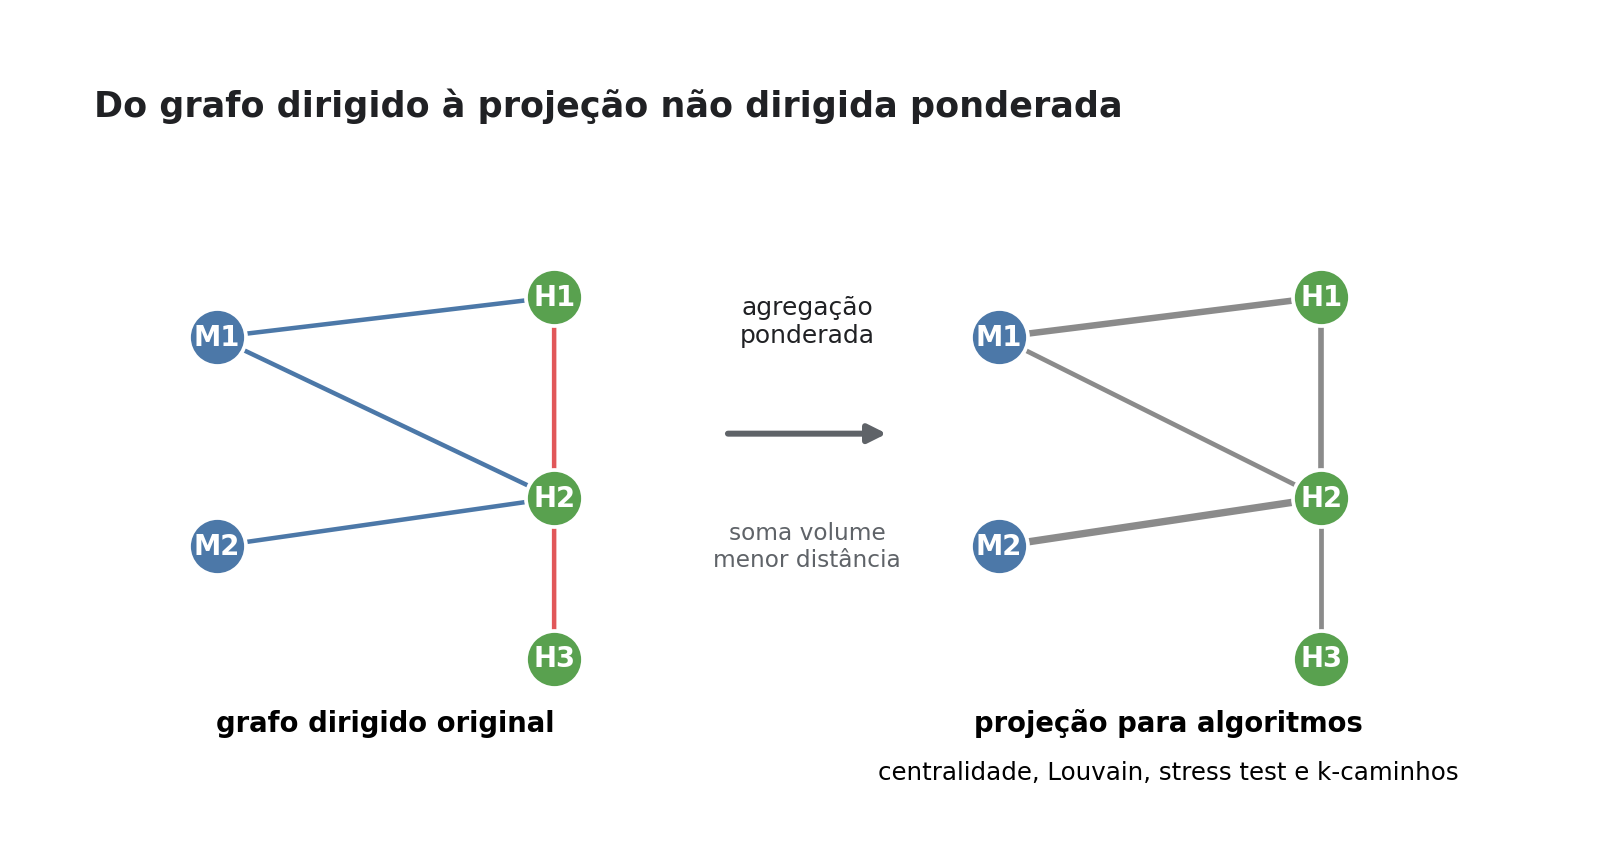
\includegraphics[width=0.62\linewidth]{figures/directed_projection.png}
\caption{Passagem do grafo dirigido de fluxos para a projeção não dirigida ponderada usada pelos algoritmos de conectividade.}
\label{fig:projecao}
\end{figure}

A validação combinou testes automatizados e reconciliação de totais. Os testes cobrem seleção SIH, contratos de esquema, enriquecimento de nós, filtros, construção do recorte público e algoritmos. Além disso, os totais do grafo, das tabelas públicas e dos relatórios finais foram comparados por arquivos de resumo JSON. Essa estratégia não elimina limitações dos dados públicos, mas torna as transformações auditáveis.

\section{Algoritmos e Resultados}

\subsection{Centralidade de Intermediação}

A centralidade de intermediação (\textit{betweenness centrality}) mede quanto um vértice aparece em caminhos mínimos entre outros pares de vértices \cite{freeman1977,brandes2001}. No contexto do projeto, um hospital com alta intermediação não é apenas um hospital com grande volume; ele atua como ponte entre municípios, regiões e corredores de atendimento. A distância foi usada como custo dos caminhos, a métrica foi normalizada e a execução usou aproximação por amostragem com \texttt{k=200} nós e semente aleatória 42, para viabilizar a execução em máquina local.

\begin{lstlisting}[caption={Centralidade de intermediação em hospitais públicos.}]
G = maior componente da projecao ponderada
calcular betweenness em G usando distancia_km como custo
selecionar apenas vertices do tipo hospital
ordenar hospitais por betweenness decrescente
\end{lstlisting}

\begin{figure}[tbp]
\centering
\begin{subfigure}[t]{0.49\linewidth}
\centering
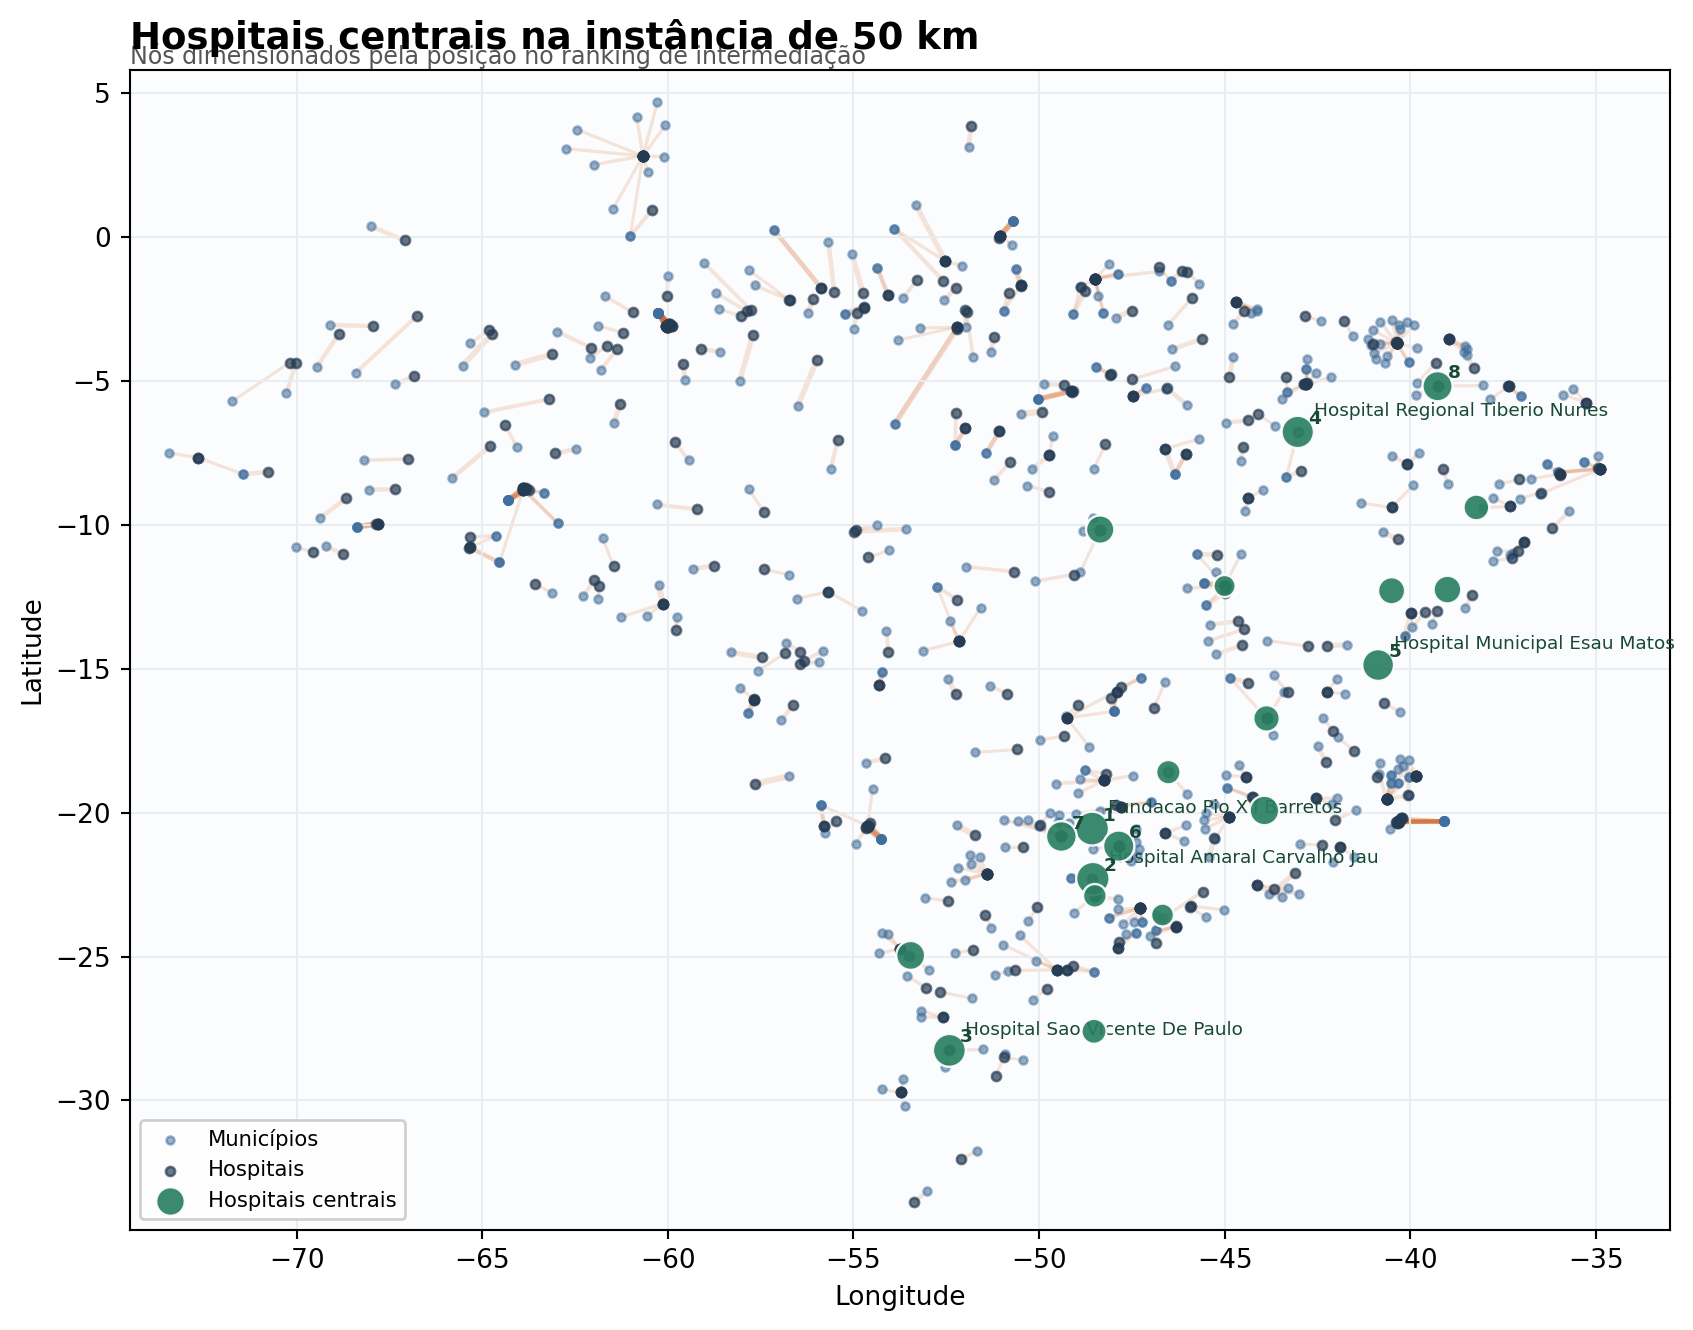
\includegraphics[width=\linewidth]{figures/map_central_hospitals.png}
\caption{Distribuição espacial no corte de 50 km.}
\label{fig:mapa-centralidade}
\end{subfigure}\hfill
\begin{subfigure}[t]{0.49\linewidth}
\centering
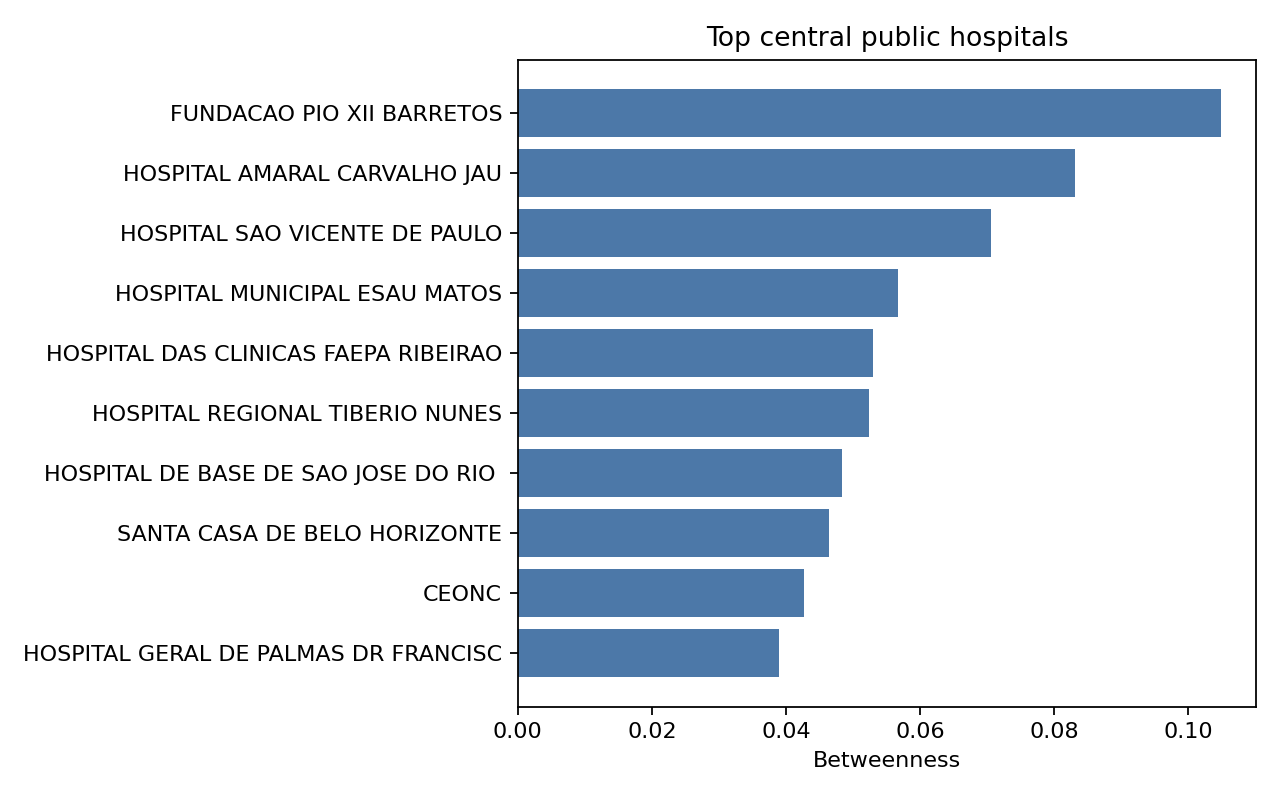
\includegraphics[width=\linewidth]{../viz_layer/reports/top_central_facilities_public_hospitals.png}
\caption{Hospitais com maior intermediação.}
\end{subfigure}
\caption{Hospitais públicos com maior centralidade de intermediação nas instâncias finais.}
\label{fig:centralidade}
\end{figure}

No corte de 50 km, os principais hospitais por centralidade foram Fundação Pio XII Barretos, Hospital Amaral Carvalho Jaú, Hospital São Vicente de Paulo, Hospital Regional Tibério Nunes, Hospital Municipal Esaú Matos, Hospital das Clínicas FAEPA Ribeirão Preto e Hospital de Base de São José do Rio Preto. Parte desses estabelecimentos é reconhecida publicamente como hospital especializado, universitário ou regional \cite{hospital_amor,amaral_carvalho,hcrp,hb_riopreto}. A centralidade, portanto, reforça a ideia de polos estruturais: alguns hospitais organizam fluxos em escala superior ao município onde estão localizados.

\subsection{Comunidades Louvain}

O método Louvain agrupa vértices que têm conexões internas mais fortes do que conexões com o restante da rede \cite{blondel2008}. A métrica otimizada é a modularidade; no projeto, o peso das arestas foi o volume agregado e a execução usou semente 42. As comunidades não foram tratadas como regiões oficiais, mas como regiões funcionais sugeridas pelos próprios fluxos.

\begin{figure}[tbp]
\centering
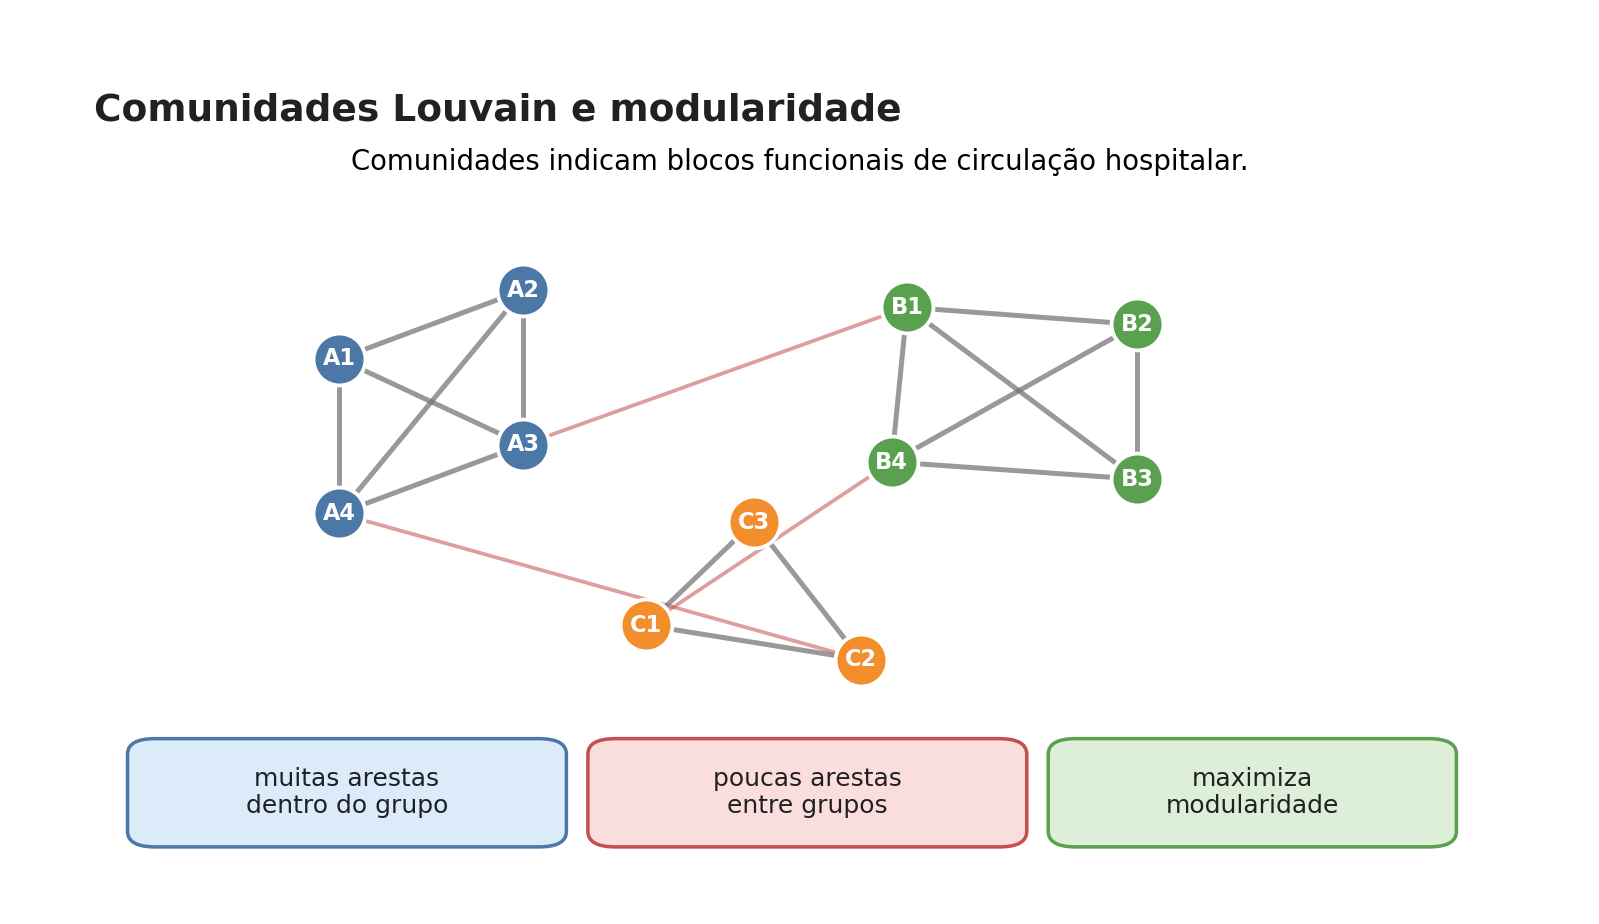
\includegraphics[width=0.60\linewidth]{figures/louvain_concept.png}
\caption{Intuição do Louvain: comunidades concentram muitas arestas internas e poucas arestas entre grupos, maximizando modularidade.}
\label{fig:louvain}
\end{figure}

As instâncias principais tiveram 49 comunidades no corte de 25 km e 43 comunidades no corte de 50 km. A redução ocorre porque o corte de 50 km remove parte dos deslocamentos regionais curtos e deixa uma rede mais seletiva, concentrada em corredores longos. A comparação com UFs e regiões de saúde foi usada como evidência descritiva de alinhamento ou desalinhamento entre rede funcional e divisão administrativa; ela não prova equivalência entre comunidade e região oficial.

\begin{figure}[tbp]
\centering
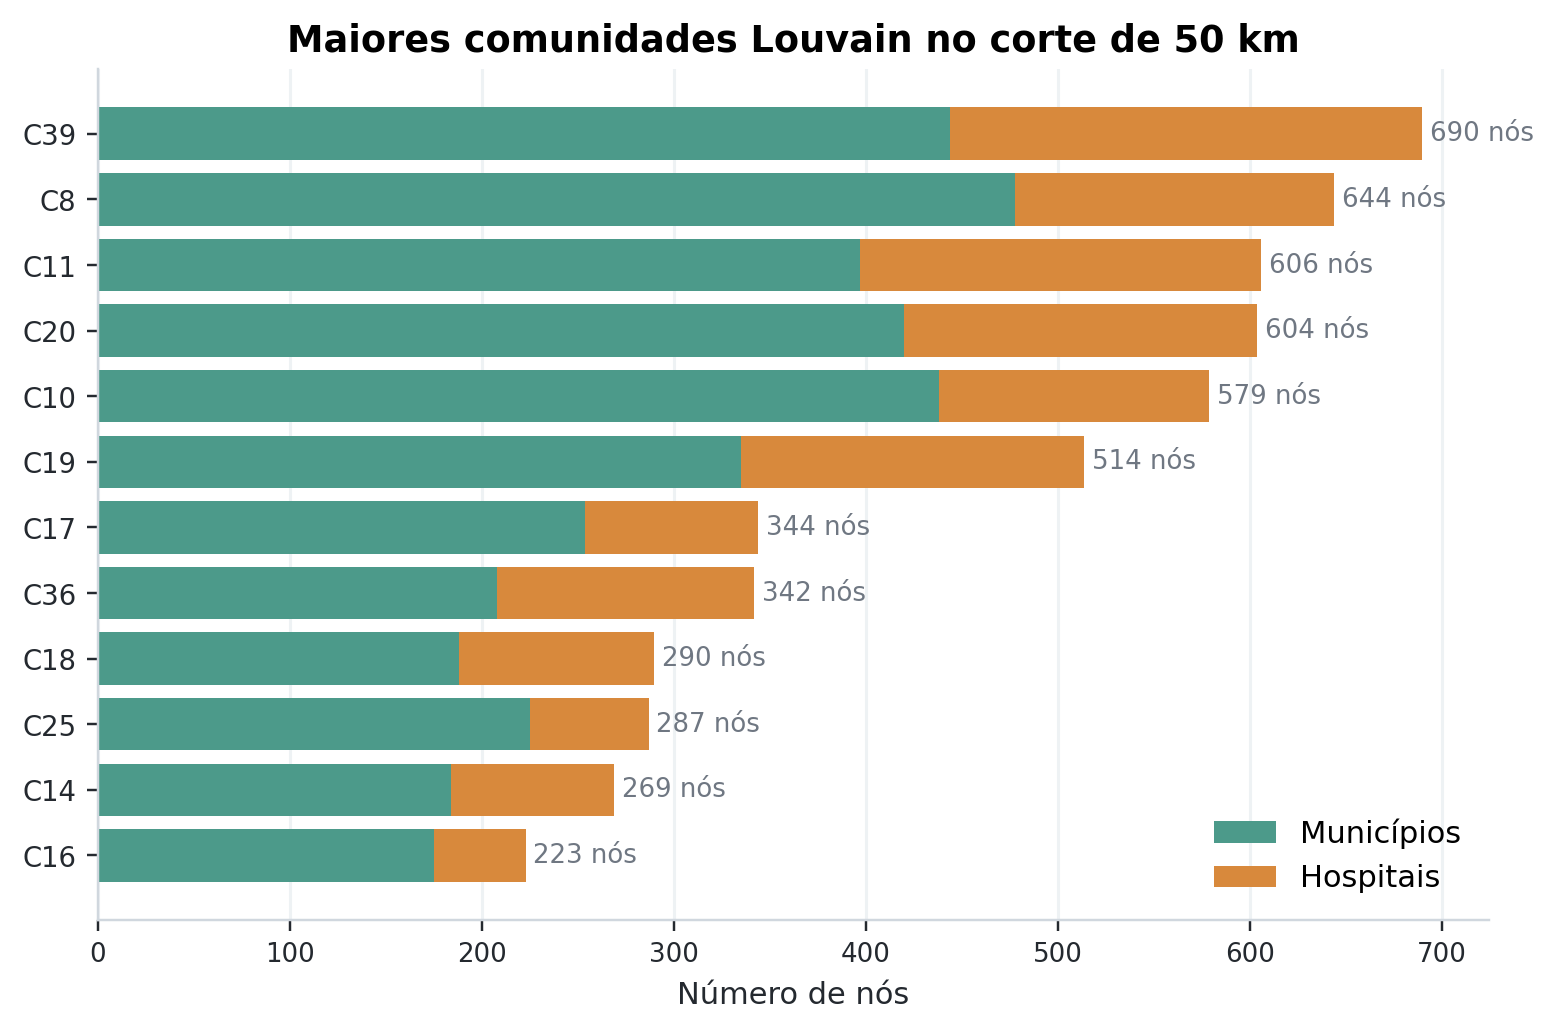
\includegraphics[width=0.64\linewidth]{figures/communities_summary_50km.png}
\caption{Maiores comunidades Louvain no corte de 50 km, separando municípios e hospitais. Comunidades maiores misturam muitos municípios de origem com um conjunto menor de hospitais de referência.}
\label{fig:comunidades-resumo}
\end{figure}

\subsection{Supressão Dinâmica}

O teste de supressão remove iterativamente hospitais com maior intermediação e recalcula a maior componente e o caminho médio amostrado. A pergunta não é se a rede ``deixa de existir'', mas se a retirada de polos centrais alonga caminhos ou fragmenta a conectividade. Em cada passo, a centralidade foi recalculada com \texttt{k=200}; o caminho médio foi estimado sobre uma amostra fixa de até 120 nós da maior componente, usando distância em km como custo.

\begin{figure}[tbp]
\centering
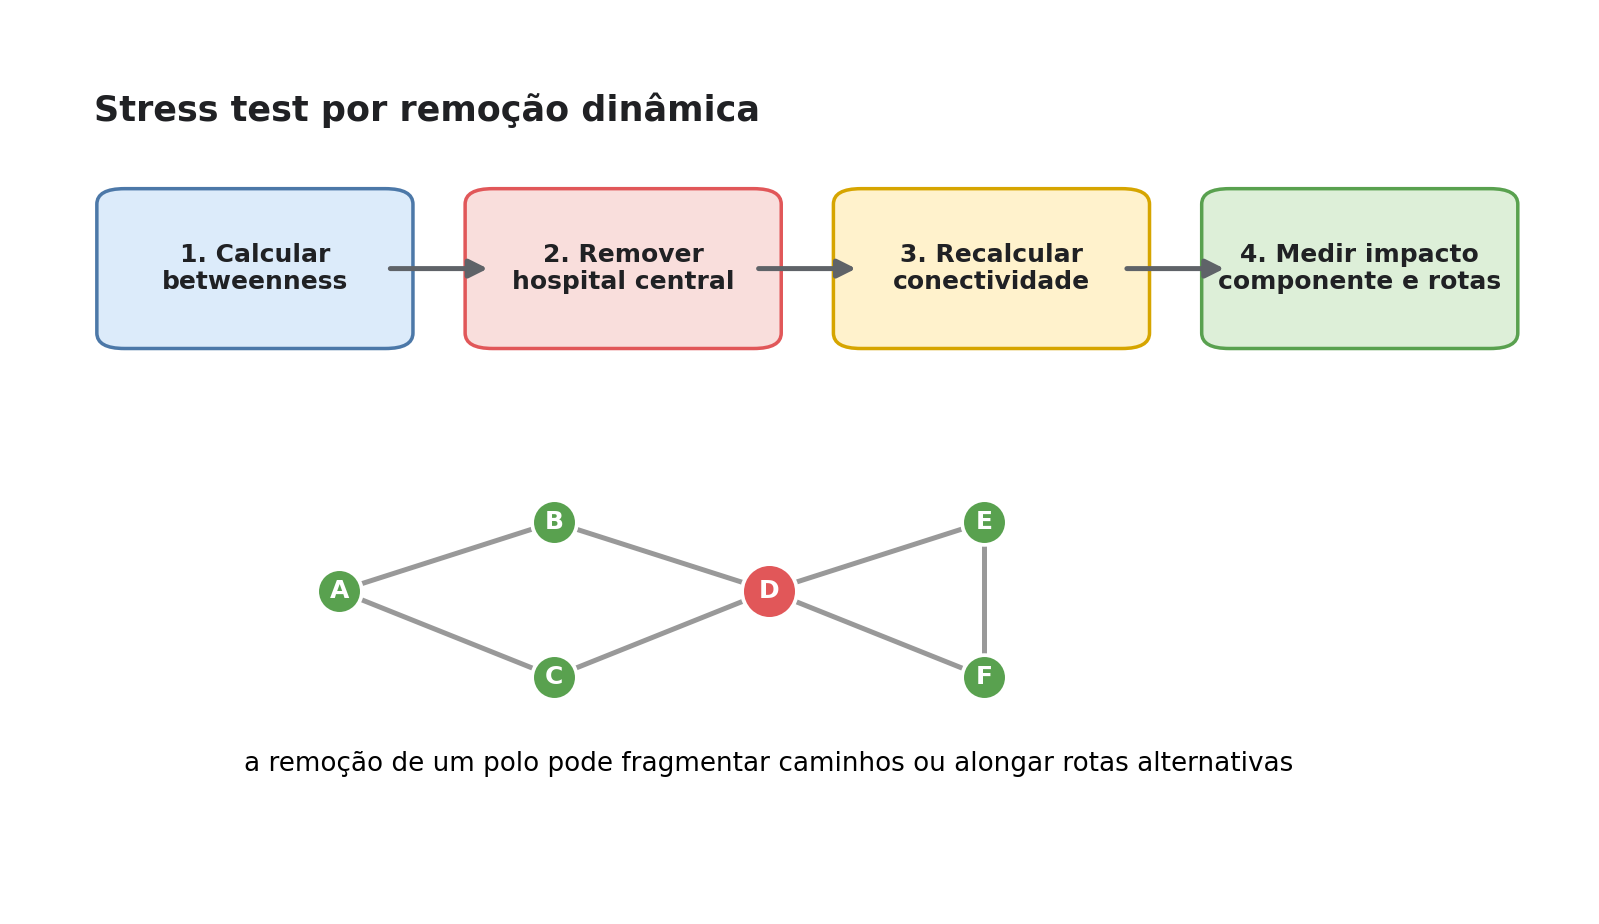
\includegraphics[width=0.60\linewidth]{figures/stress_test_algorithm.png}
\caption{Procedimento do teste de supressão dinâmica: recalcular intermediação, remover um polo e medir o efeito sobre conectividade e rotas.}
\label{fig:stress-algoritmo}
\end{figure}

\begin{lstlisting}[caption={Teste de supressão dinâmica.}]
G = maior componente da instancia filtrada
registrar tamanho da componente e caminho medio amostrado
para passo em 1..5:
  recalcular betweenness dos hospitais em G
  remover hospital com maior betweenness
  recalcular maior componente e caminho medio amostrado
\end{lstlisting}

\begin{figure}[tbp]
\centering
\begin{subfigure}[t]{0.49\linewidth}
\centering
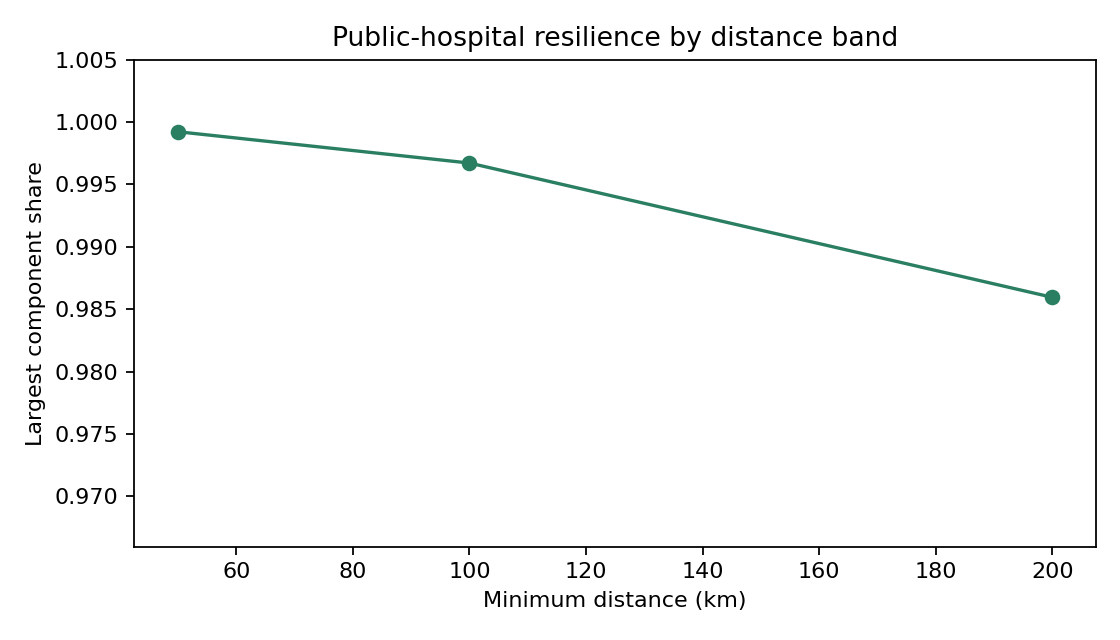
\includegraphics[width=\linewidth]{../viz_layer/reports/resilience_largest_component_public_hospitals.png}
\caption{Maior componente.}
\end{subfigure}\hfill
\begin{subfigure}[t]{0.49\linewidth}
\centering
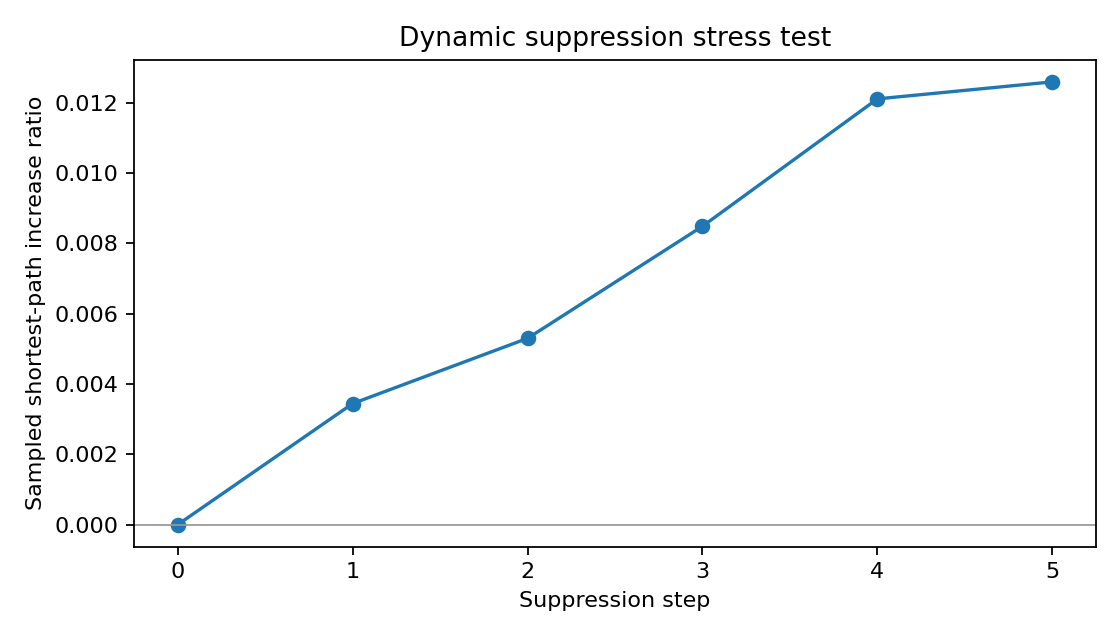
\includegraphics[width=\linewidth]{../viz_layer/reports/resilience_stress_path_increase_public_hospitals.png}
\caption{Caminho médio amostrado.}
\end{subfigure}
\caption{Efeito da supressão de hospitais centrais sobre maior componente e caminho médio amostrado.}
\label{fig:stress}
\end{figure}

\begin{table}[tbp]
\centering
\caption{Resumo das instâncias e do stress test após cinco remoções.}
\label{tab:instancias}
\begin{tabular}{lrrrrr}
\toprule
Instância & Nós & Arestas & Comunidades & Maior comp. final & Aumento caminho \\
\midrule
25 km & 8.622 & 61.706 & 49 & 99,9072\% & 0,7839\% \\
50 km & 7.750 & 47.739 & 43 & 99,4702\% & 1,2597\% \\
\bottomrule
\end{tabular}
\end{table}

O resultado agregado indica que a rede nacional não se fragmenta facilmente. Porém, essa conclusão precisa ser lida com cuidado: conectividade nacional não mede disponibilidade de vaga, tempo real de deslocamento ou impacto local. A rede pode preservar 99\% da maior componente enquanto um município específico perde seu destino de referência. Por isso, o stress test é mais útil como contraste: ele mostra robustez global, e essa robustez torna ainda mais necessário olhar dependências municipais.

\subsection{K-Caminhos Mais Curtos}

Os k-caminhos mais curtos (\textit{k-shortest paths}) foram usados para avaliar redundância topológica \cite{dijkstra1959,yen1971}. Em vez de perguntar apenas qual é o menor caminho entre uma origem e um hospital, o método pergunta quais seriam as próximas melhores conexões na projeção não dirigida. Assim, para um par município $\rightarrow$ hospital de alto volume, calculamos o melhor caminho $k_1$ e, quando existente, um segundo caminho $k_2$ que não repete exatamente a mesma sequência de nós. A razão $d(k_2)/d(k_1)$ indica o custo relativo da alternativa topológica.

Essa leitura é importante porque conectividade não significa substituição fácil. Se $k_2$ tem distância parecida com $k_1$, há redundância topológica próxima. Se $k_2$ é duas, três ou cinco vezes mais longo, a rede até possui uma alternativa no grafo, mas ela pode ser ruim como opção assistencial. Quando apenas um caminho foi encontrado na instância filtrada, o par foi marcado como sem alternativa relevante dentro dos critérios de recorrência e distância adotados.

No corte de 50 km foram avaliados os 30 pares residência $\rightarrow$ hospital de maior volume, buscando até 3 caminhos por par. Em 1 caso não houve segunda alternativa; entre os 29 pares restantes, 27 tiveram razão $d(k_2)/d(k_1)$ acima de 2, com média 3,05 e máximo 6,34. Isso mostra que redundância não é binária: uma região pode estar conectada no grafo e ainda assim depender de alternativas longas ou frágeis.

\begin{figure}[tbp]
\centering
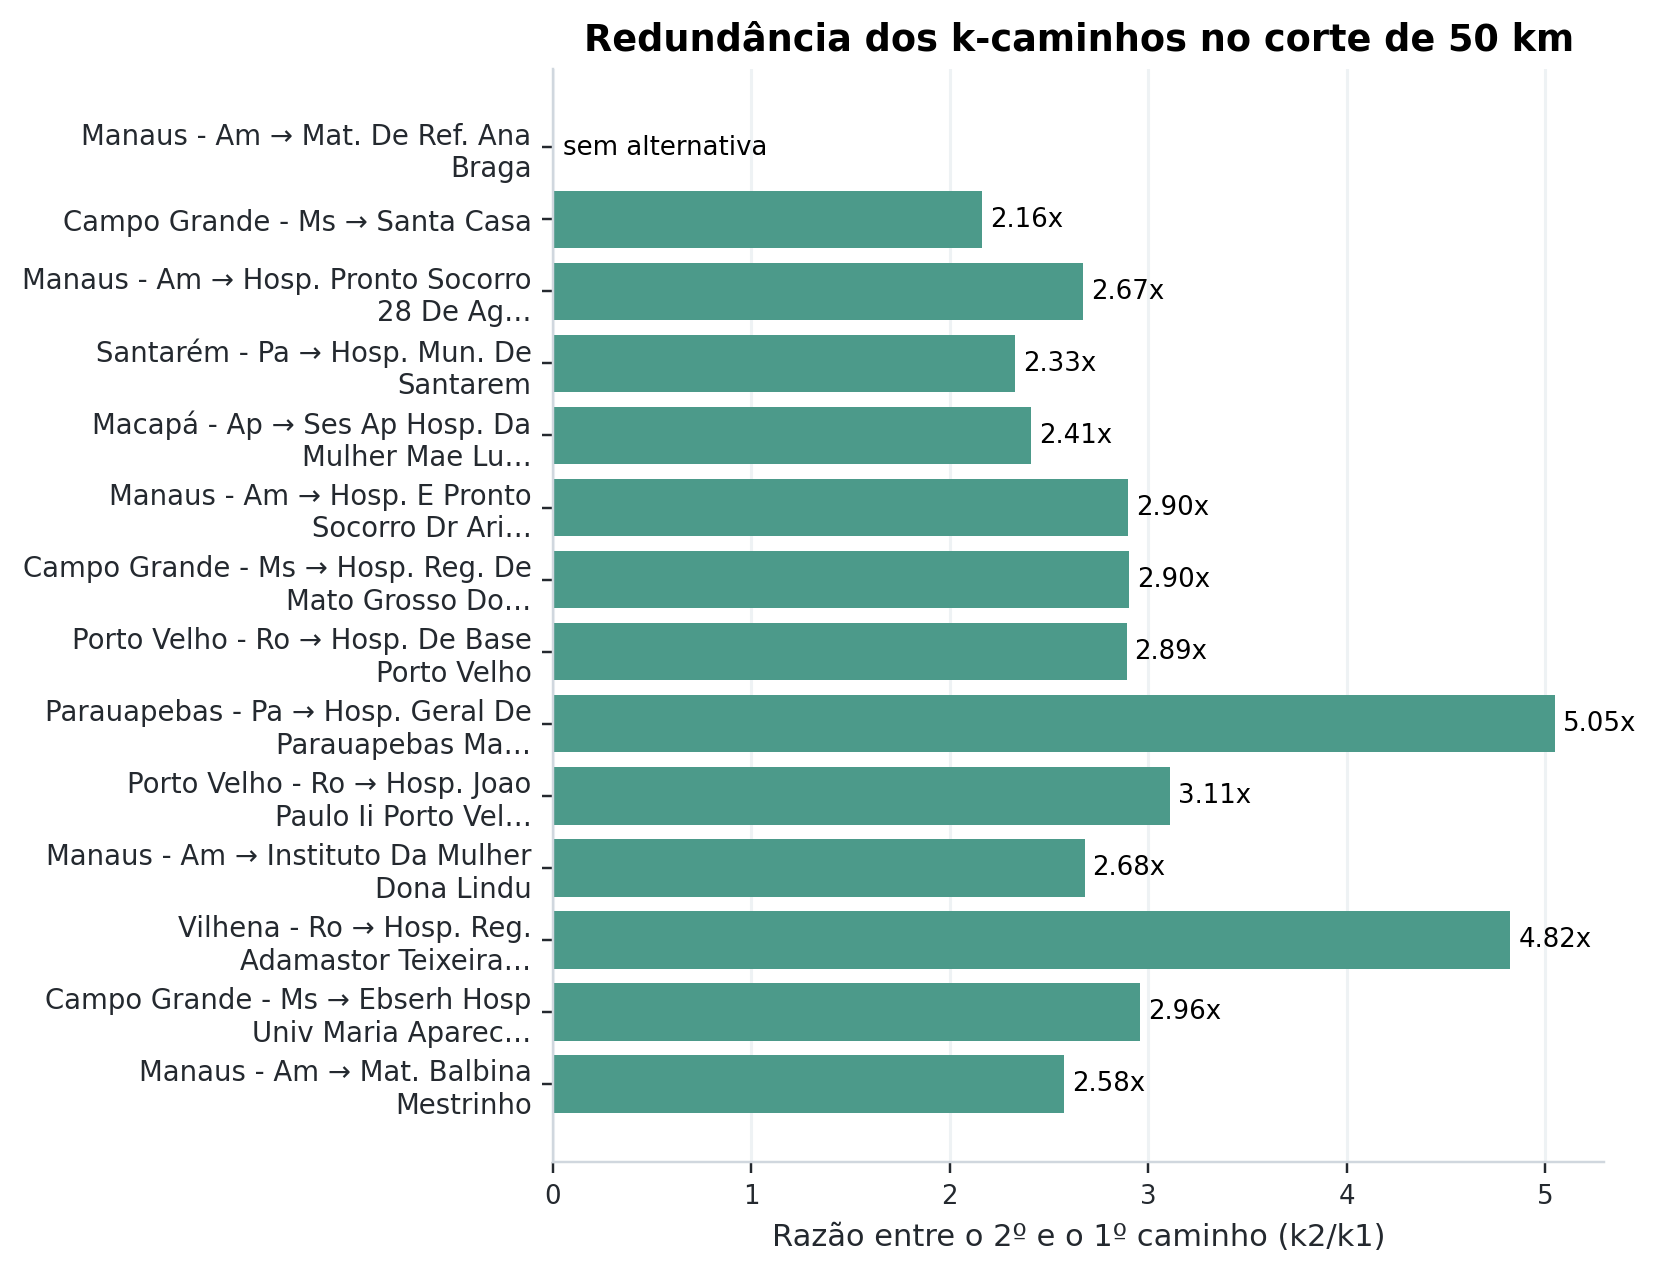
\includegraphics[width=0.68\linewidth]{figures/k_path_redundancy.png}
\caption{Razão entre o segundo e o primeiro caminho mais curto em pares de alto volume no corte de 50 km. Valores acima de 2 indicam alternativas formalmente existentes, mas possivelmente pouco substitutivas.}
\label{fig:k-caminhos}
\end{figure}

\FloatBarrier

\section{Regiões Oficiais e Dependência Municipal}

A comparação regional usou o campo \texttt{REGSAUDE} dos arquivos CNES/ST de janeiro de 2021. A referência cobriu 27 arquivos estaduais, 334.702 linhas CNES e 5.570 municípios, mas também registrou 1.250 municípios com conflito de código regional entre estabelecimentos e 239 sem região identificada. Por isso, a regionalização foi tratada como aproximação oficial baseada no CNES, não como verdade administrativa perfeita. A parcela ``fora da região'' usa o fluxo total filtrado como denominador; a coluna de região ignorada explicita quanto desse total não pôde ser classificado.

\begin{table}[tbp]
\centering
\caption{Fluxos recorrentes que cruzam região oficial de saúde.}
\label{tab:regioes}
\scriptsize
\begin{tabular}{llrrrrrr}
\toprule
Dist. & Tipo & Arestas & Fluxo total & Fora região & Parcela & Região ign. & Dist. média \\
\midrule
25 km & Residência & 60.646 & 3.488.440 & 1.117.796 & 32,04\% & 204.219 & 86,96 km \\
25 km & Transferência & 1.060 & 3.585 & 1.868 & 52,11\% & 160 & 148,14 km \\
50 km & Residência & 46.938 & 1.942.302 & 850.778 & 43,80\% & 137.170 & 128,20 km \\
50 km & Transferência & 801 & 2.748 & 1.676 & 60,99\% & 104 & 182,08 km \\
\bottomrule
\end{tabular}
\end{table}

A Tabela \ref{tab:regioes} concentra um dos achados centrais. Aqui, ``fora da região'' não significa necessariamente sair do estado. A comparação usa a região oficial de saúde do CNES, identificada pelo campo \texttt{REGSAUDE}; um mesmo estado possui várias regiões de saúde, por isso muitos cruzamentos aparecem como PE-0004 $\rightarrow$ PE-0001, SP-0201 $\rightarrow$ SP-0101 ou BA-0003 $\rightarrow$ BA-0001. Esses são fluxos entre regiões administrativas diferentes dentro da mesma UF. Cruzamentos de estado também existem e foram calculados separadamente como \textit{cross UF}; no corte de 50 km, eles representaram 3,32\% do fluxo residência $\rightarrow$ hospital e 1,42\% do fluxo hospital $\rightarrow$ hospital, portanto não explicam a maior parte dos cruzamentos regionais.

Quando os fluxos são recorrentes, parte expressiva do atendimento ultrapassa a região oficial de saúde. Isso não significa que todo deslocamento inter-regional seja problemático: alta complexidade frequentemente exige referência externa. O sinal de vulnerabilidade aparece quando o deslocamento é repetido, longo e concentrado em poucos destinos.

\begin{figure}[tbp]
\centering
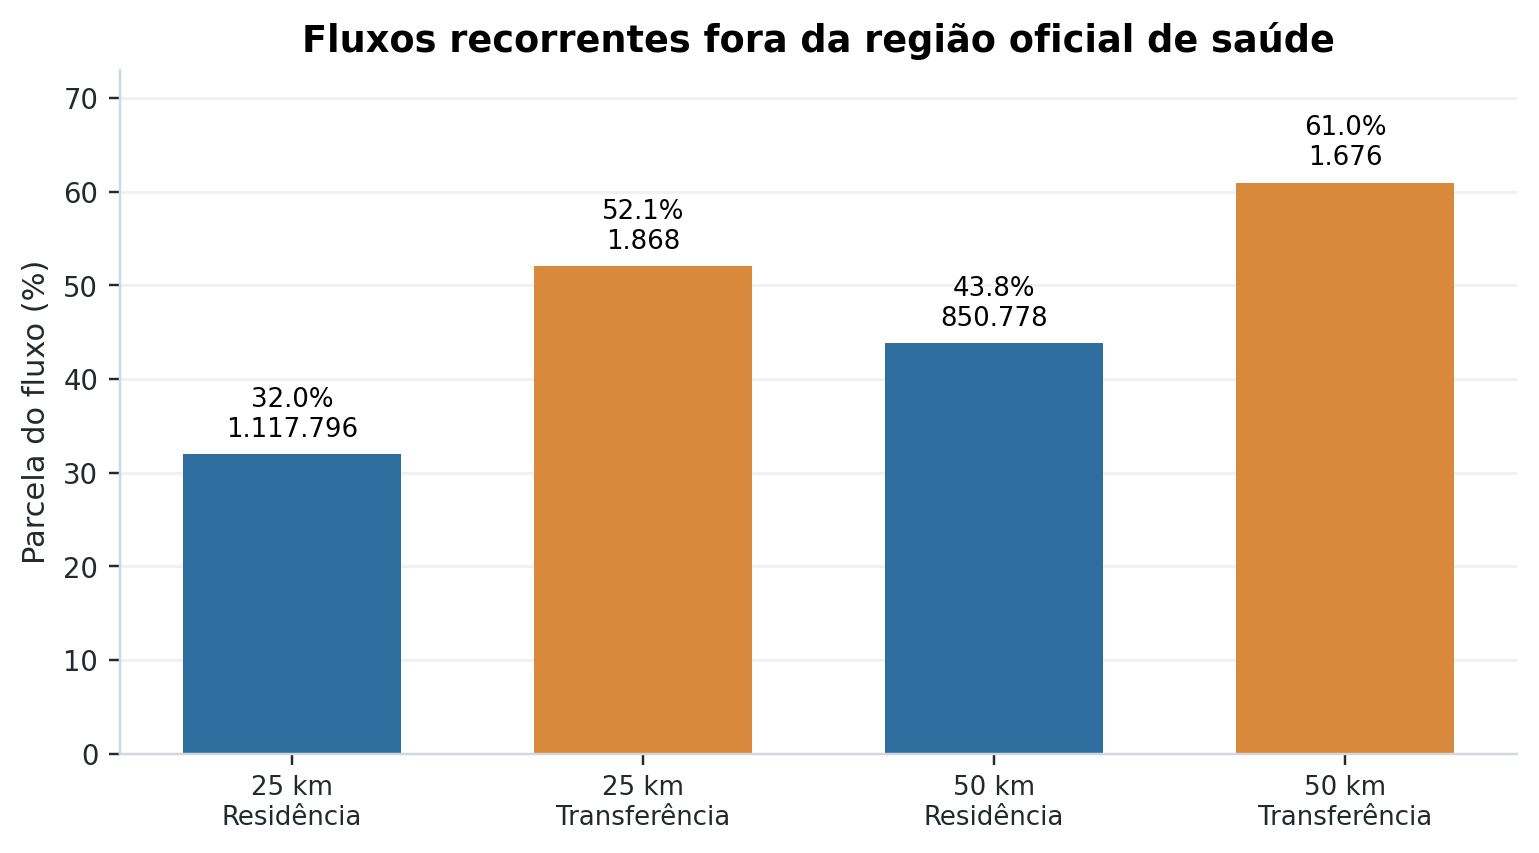
\includegraphics[width=0.66\linewidth]{figures/regional_cross_share.png}
\caption{Parcela do fluxo recorrente que cruza regiões oficiais de saúde, por tipo de aresta e limiar de distância.}
\label{fig:fluxos-fora-regiao}
\end{figure}

\begin{figure}[tbp]
\centering
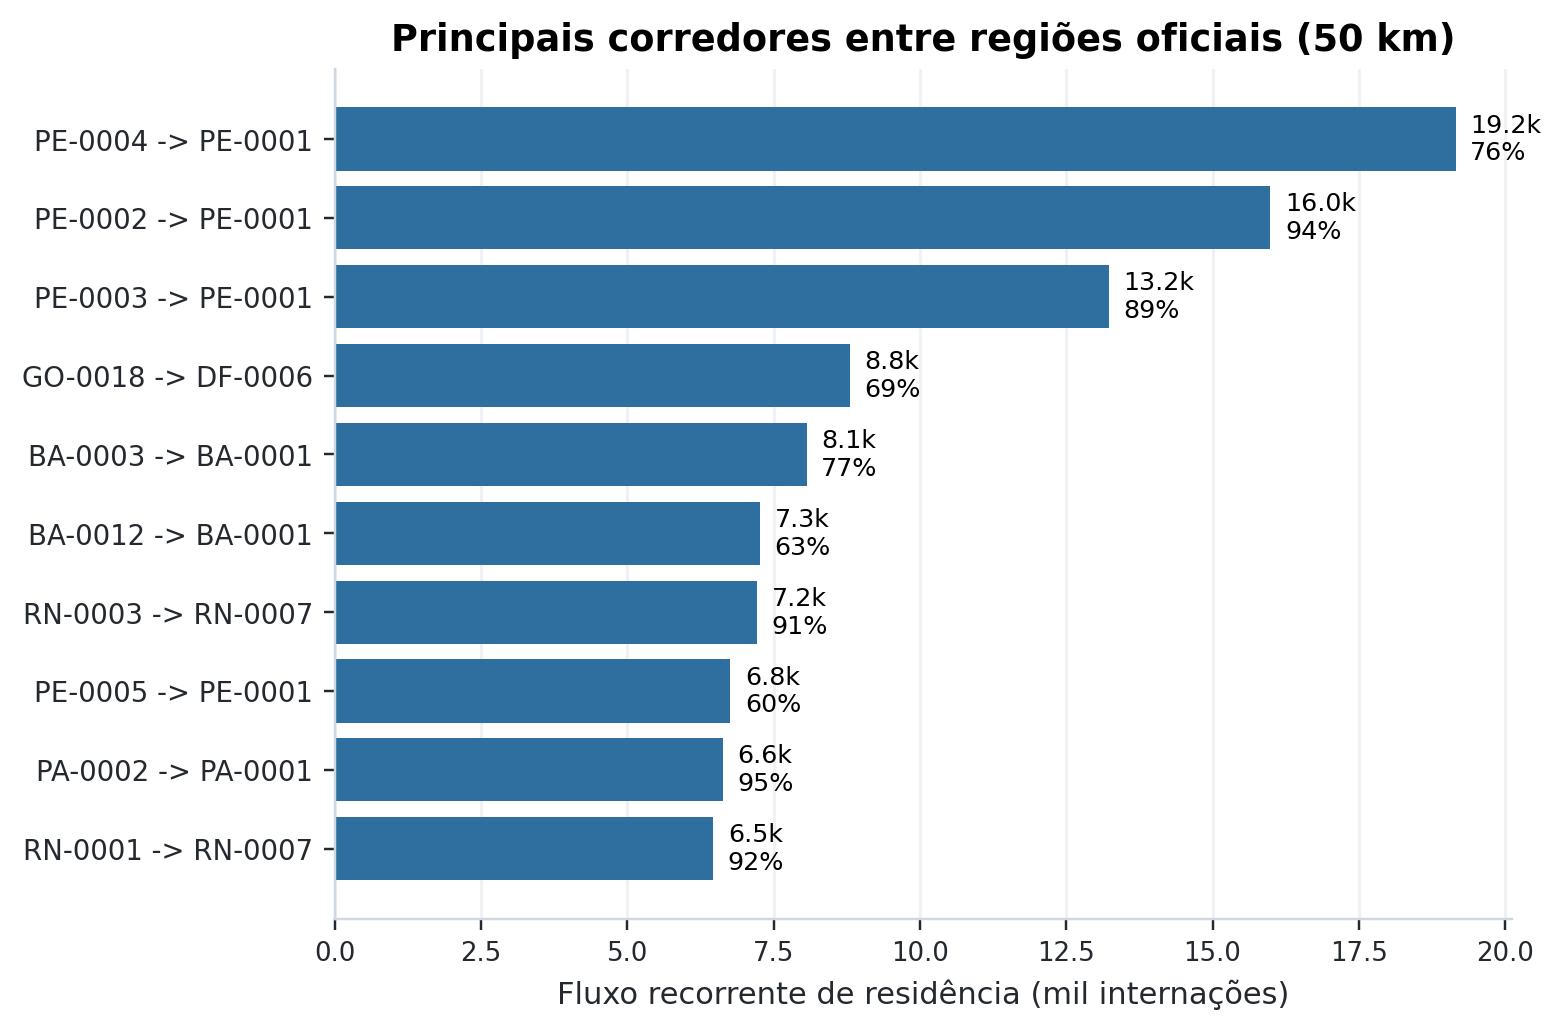
\includegraphics[width=0.68\linewidth]{figures/regional_mismatch_top.png}
\caption{Principais corredores região $\rightarrow$ região no corte de 50 km. Os códigos seguem a UF e o identificador regional do CNES; a anotação ao lado das barras indica também a participação do corredor no fluxo de origem.}
\label{fig:corredores-regionais}
\end{figure}

\begin{table}[tbp]
\centering
\caption{Exemplos de dependência municipal no corte de 50 km. A participação refere-se ao fluxo filtrado recorrente e distante, não ao total de internações do município.}
\label{tab:dependencia}
\scriptsize
\begin{tabularx}{\linewidth}{L{0.22\linewidth}Yrrr}
\toprule
Município & Principal destino externo & Fluxo & Participação & Distância \\
\midrule
Serra Nova Dourada -- MT & Hospital Regional de Água Boa & 96 & 100\% & 241,2 km \\
Caiana -- MG & Hospital do Câncer de Muriaé & 70 & 100\% & 65,4 km \\
Dom Cavati -- MG & Hospital Municipal Eliane Martins & 58 & 100\% & 50,1 km \\
Bujaru -- PA & Hospital Regional Público Dr. Abelardo Santos & 47 & 100\% & 56,1 km \\
Santana do Cariri -- CE & Hospital Maternidade São Vicente de Paulo & 41 & 100\% & 50,8 km \\
\bottomrule
\end{tabularx}
\end{table}

Esses exemplos foram selecionados pela ordenação do relatório de dependência: corte de 50 km, fluxo recorrente, destino principal concentrando 100\% do fluxo filtrado e cruzamento de região oficial. Eles mostram por que a média nacional é insuficiente. Para a rede inteira, uma remoção pode alterar pouco a maior componente; para um município que concentra todo o fluxo filtrado em um destino fora de sua região, a perda desse destino representa uma fragilidade concreta dentro dos critérios adotados. Em um estudo mais focalizado, uma extensão natural seria escolher um estado ou macrorregião, validar a regionalização com bases locais e analisar impactos percentuais por município e especialidade.

\section{Visualização}

A visualização final foi desenhada como camada de apresentação analítica, não como tentativa de renderizar todas as 188 mil arestas no navegador. O script \ghfile{viz_layer/build_final_map_layers.py}{build\_final\_map\_layers.py} gera o arquivo leve \ghfile{viz_layer/reports/final_map_layers.json}{final\_map\_layers.json}, com corredores principais, hospitais centrais, nós removidos no stress test, comunidades e exemplos de dependência municipal.

No \ghfile{viz_layer/graph_map_ui.html}{graph\_map\_ui.html}, o usuário pode alternar presets de 25 km, 50 km, hospitais centrais, stress test e dependência municipal. A interface evita desenhar tudo ao mesmo tempo: trabalha com camadas reduzidas, oculta arestas durante navegação e redesenha em blocos. Essa decisão foi necessária porque a visualização bruta ficava pesada, enquanto a versão guiada preserva a mensagem analítica e roda em computadores comuns. Como alternativa estática, \ghfile{viz_layer/reports/final_showcase.html}{final\_showcase.html} reúne gráficos e tabelas principais.

\begin{figure}[tbp]
\centering
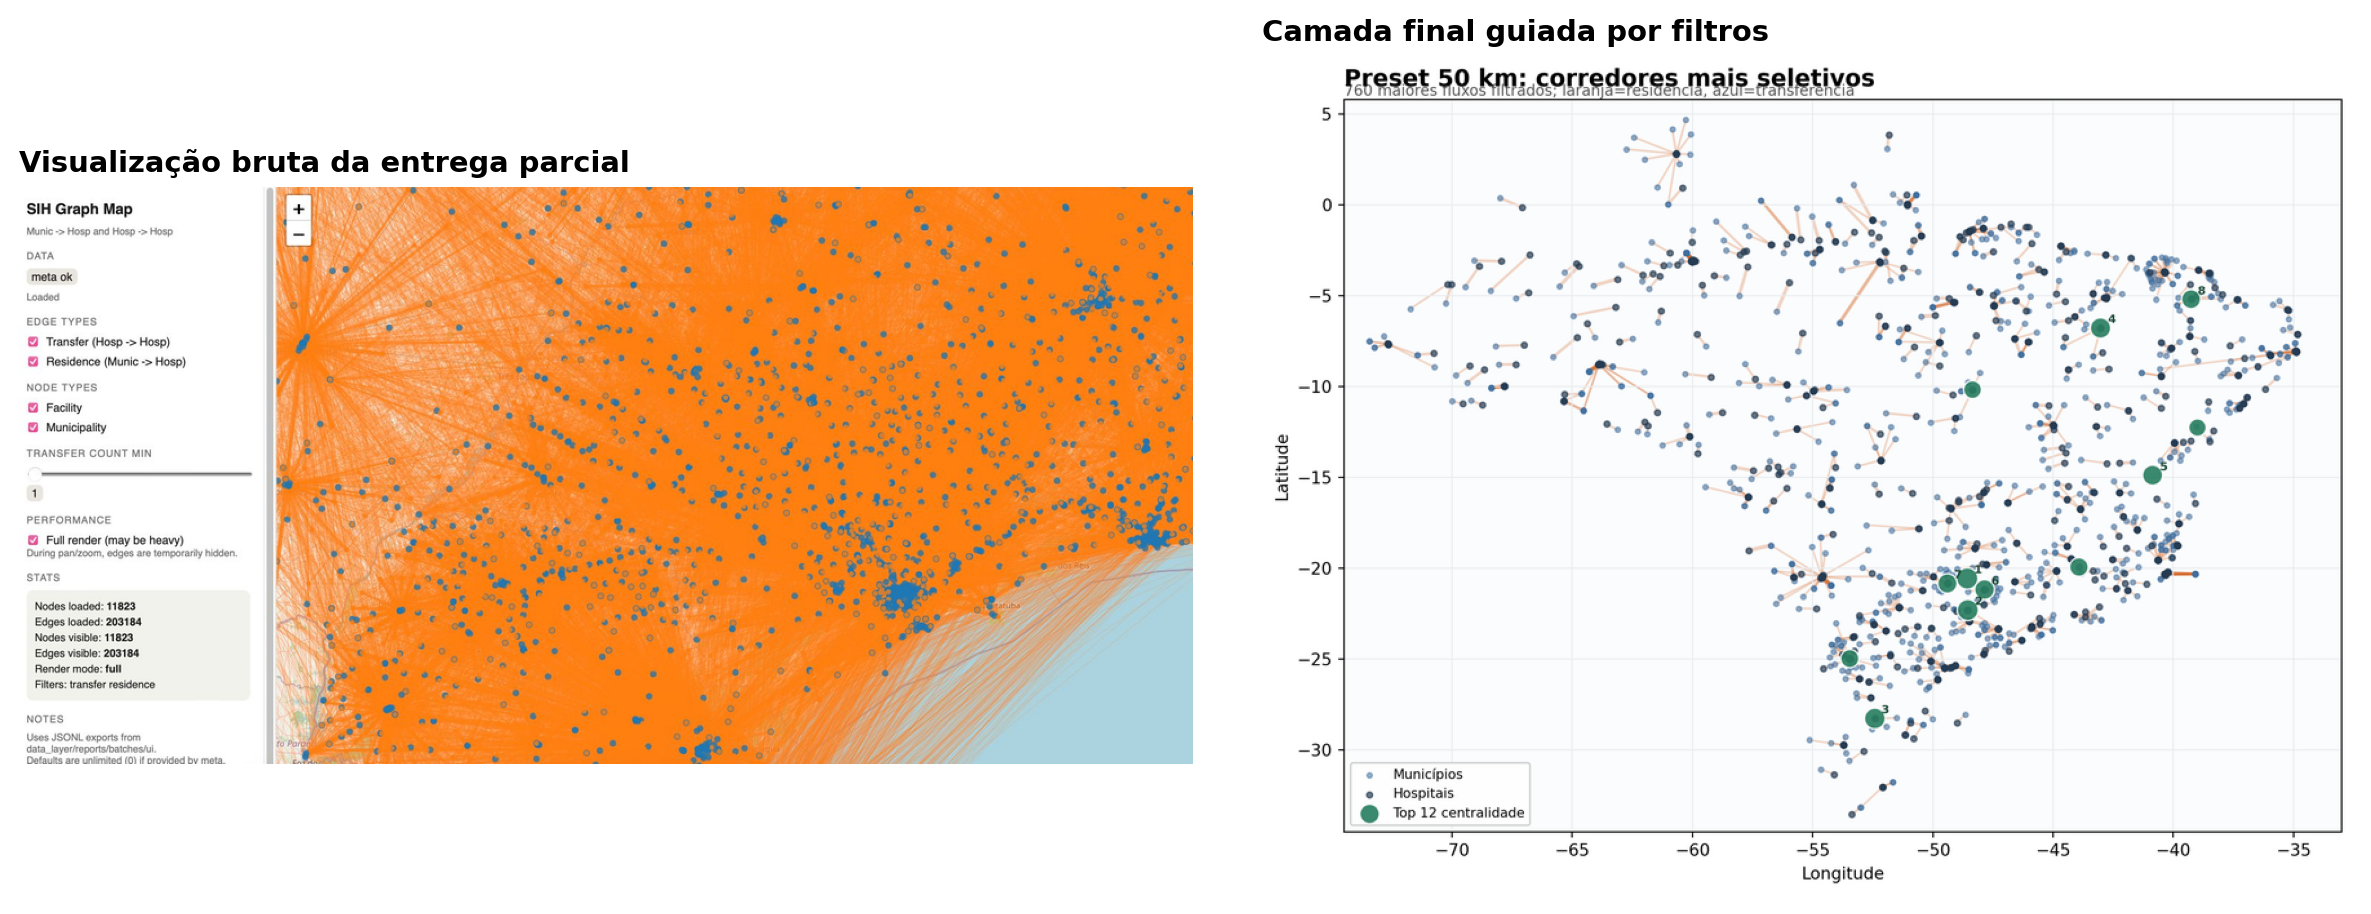
\includegraphics[width=0.86\linewidth]{figures/visual_raw_vs_guided.png}
\caption{Comparação entre a visualização bruta da entrega parcial e a camada final guiada por filtros. A decisão de não renderizar todas as arestas ao mesmo tempo foi necessária para manter legibilidade e desempenho.}
\label{fig:raw-vs-guided}
\end{figure}

\begin{figure}[tbp]
\centering
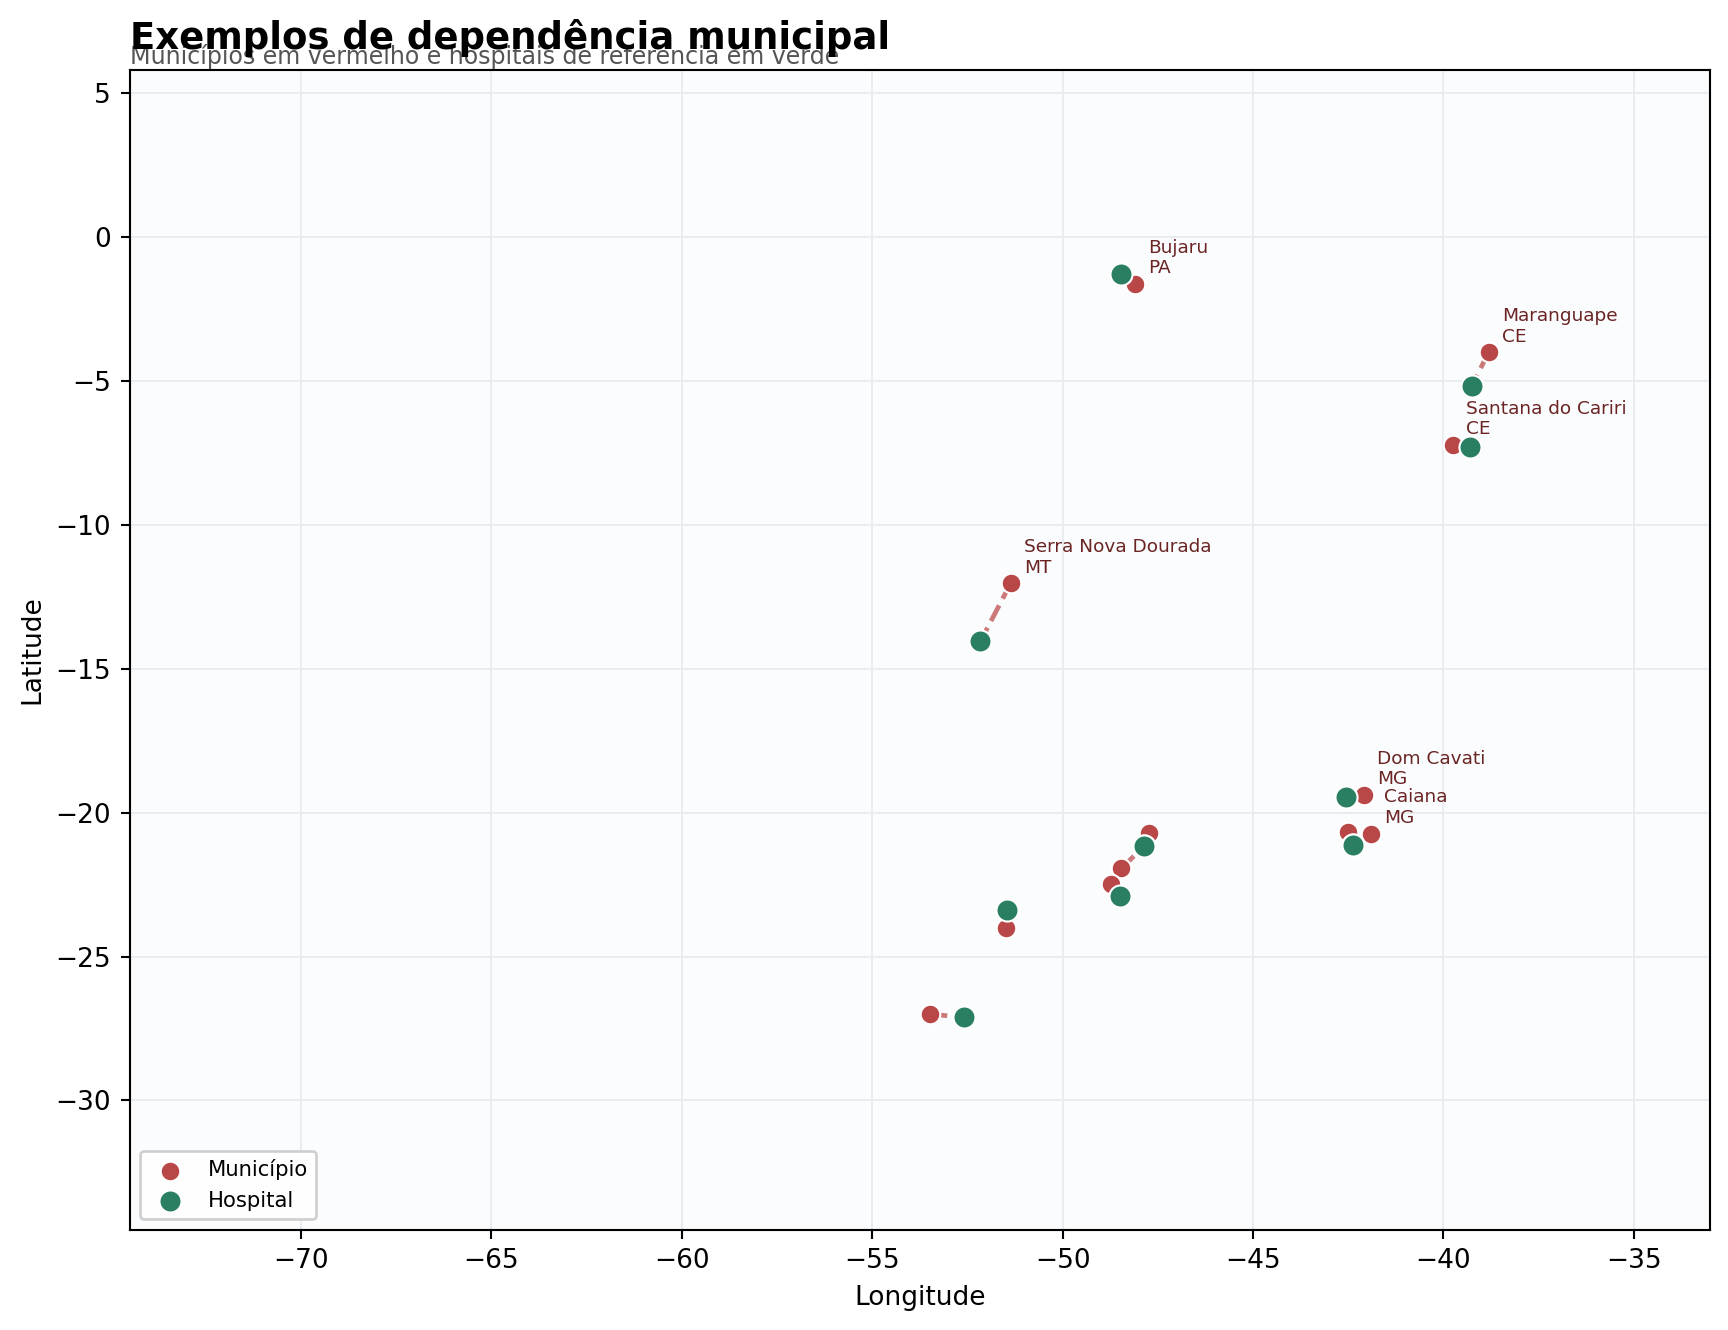
\includegraphics[width=0.56\linewidth]{figures/map_dependency_examples.png}
\caption{Exemplos geográficos de dependência municipal usados pela camada de visualização final.}
\label{fig:mapa-dependencias}
\end{figure}

\FloatBarrier

\section{Limitações e Interpretação}

Os resultados devem ser interpretados como análise de acesso realizado, não de necessidade total. O SIH mostra internações que ocorreram; ele não mostra pacientes que não conseguiram vaga, demanda reprimida ou tempo de espera. Além disso, a base anual não mede capacidade simultânea: volume em 2021 não informa quantos leitos estavam disponíveis em uma semana crítica, quais equipes estavam ativas ou quais especialidades eram necessárias. Como 2021 ainda foi marcado pela pandemia de COVID-19, parte dos fluxos pode refletir reorganizações emergenciais da rede.

Outra limitação é espacial. A distância Haversine aproxima deslocamento em linha geodésica, mas não mede tempo por estrada, transporte público, rios ou barreiras locais. Em áreas rurais e amazônicas, 50 km podem representar realidades muito diferentes. A inferência de transferências também é probabilística e conservadora; ela é útil para padrões estruturais, mas não substitui uma base clínica de regulação com identificadores explícitos de origem e destino. Como não houve validação individual de prontuário ou regulação, as arestas de transferência devem ser lidas como sinal agregado de continuidade provável, não como verdade clínica.

Por fim, a análise regional depende do \texttt{REGSAUDE} disponível no CNES/ST. Como foram encontrados conflitos e ausências, a comparação com regiões oficiais é uma aproximação. Além disso, os algoritmos de conectividade operam sobre uma projeção não dirigida: ela é útil para estudar estrutura, mas não preserva todas as restrições direcionais e administrativas do atendimento real. Ainda assim, o volume de fluxos fora da região é suficientemente alto para indicar uma tensão entre o desenho administrativo e os caminhos observados nos dados.

\section{Conclusão}

O projeto transformou dados públicos de internação em uma rede nacional documentada, filtrável, analisável e visualizável. A implementação entregou não apenas o grafo, mas também camadas de validação, tabelas analíticas, algoritmos e uma interface final para explorar os resultados.

A conclusão substantiva é que a rede pública hospitalar brasileira de 2021 é conectada no agregado, mas não homogênea. Hospitais especializados e regionais aparecem como polos estruturais; fluxos recorrentes cruzam regiões oficiais de saúde; e alguns municípios dependem fortemente de poucos destinos externos. Portanto, a contribuição do trabalho não é apenas apontar hospitais grandes, mas mostrar como a estrutura dos fluxos revela dependências locais que métricas nacionais podem esconder.

Como continuidade, o projeto ganharia precisão com leitos por competência, ocupação temporal, tempo real de deslocamento, separação por especialidade e validação regional com dados locais. Um estudo focalizado em um estado de referência também permitiria medir impactos percentuais com mais sensibilidade e discutir políticas de regionalização com bases administrativas mais limpas.

\bibliographystyle{plain}
\bibliography{references}

\end{document}
